\documentclass[]{article}
\usepackage[spanish]{babel} 
\usepackage{amsmath} 
\usepackage[colorlinks=true]{hyperref}
\usepackage{enumitem} 
\usepackage{graphicx}   
\usepackage[a4paper,top=2.5cm,bottom=2.5cm,left=2cm,right=2.5cm]{geometry} 
\usepackage[]{subfigure}
\usepackage[]{multicol}
\setlength{\columnsep}{1cm}
\usepackage[]{hyperref}
%\usepackage[maxbibnames=99, sorting=none]{biblatex}
\usepackage{amssymb}
\usepackage[]{txfonts}

%\usepackage[authoryear]{natbib}
\newenvironment{Figura}
  {\par\medskip\noindent\minipage{\linewidth}}
  {\endminipage\par\medskip}


\title{Electromagnetismo} 
\author{Noemí de la Peña, Benjamín Opazo, Martina Contreras \\ \\
 \textit{ Departamento de Física, Universidad de Concepción, Concepción, Chile. }}
  \date{} 

  



   %==================================================================================
\begin{document}
\maketitle 



    


%=============Resumen============
\begin{abstract}
    En este laboratorio se llevaron a cabo 3 experimentos relacionados con el electromagnetismo:  el motor homopolar, el electroimán e inducción electromagnética.
Finalmente, se concluye lo siguiente,  cuando hay una corriente eléctrica pasando por un cable se genera un campo magnético, además si se hace variar este útimo, generará una fem\footnote[1]{Fuerza Electro Motriz}.

\end{abstract}


\begin{multicols*}{2}

%========Introducción=============
\section*{Introdución}
El descubrimiento de la electricidad sucede alrededor del siglo 600 a. C. el filósofo griego Tales de Mileto descubrió que si frotaba un trozo de la resina vegetal fósil llamada ámbar adquiría la propiedad de atraer pequeños objetos.\\
 El magnetismo, este se descubrió en la región de Magnesia, Grecia (de ahí el origen de la palabra magnética) al observar que pedazos de roca natural llamada magnetita (Fe3O4) atraen el hierro.
Estas 2 ciencias se estudiaron por separado durante siglos, no fue hasta 1820 donde un físico y químico, Hans Christian Oersted, descubriría al preparar su clase de física en la Universidad de Copenhague que a la circular corriente por un conductor se genera un campo magnético.
Este descubrimiento abrió abundantes vías de investigación sobre magnetismo y la electricidad.  
En 1831 el científico británico Michael Faraday, de los descubrimiento de Oersted, consiguió producir una corriente eléctrica a partir de una acción magnética, fenómeno conocido como inducción electromagnética.
 A partir de estos experimentos, se formularían leyes cuantitativas, tales como en 1826 la ley de Ampere, las leyes de Maxwell, ley de Lorentz (1895), la ley de Faraday y la ley Biot-Savart (1820).
 En este informe, primero definiremos algunas leyes y conceptos importantes , luego presentaremos los materiales , procedimiento y un análisis para cada uno de los experimentos realizados, para concluir con lo que hemos aprendido al realizar este laboratorio.


%==============Marco teorico============
\section*{Marco teórico}
\begin{itemize}
    \item \textbf{Ley de Loretz: }\cite{Ley-de-Lorentz}  establece que una partícula cargada $q$ que circula a una velocidad $\overrightarrow{v}$ por un punto en el que existe una 
    intensidad de campo magnético $\overrightarrow{B}$, sufrirá la acción de una fuerza $\overrightarrow{F}$ denominada \textbf{fuerza de Lorentz} cuyo valor
    es proporcional al valor de $q$, $\overrightarrow{B}$ y $\overrightarrow{v}$ se obtiene por medio de la siguiente expresión:
    
    \begin{align}
        \overrightarrow{F} =  q\overrightarrow{v} \, x \, \overrightarrow{B}.
        \label{eq: Lorentz}
    \end{align}
    
    \item \textbf{Ley de Ampère: }\cite{Ley-de-Ampere} determina que la circulación del campo magnético a lo largo de una línea cerrada es equivalente a la suma algebraica de las intensidades 
    de la corrientes que atraviesan la superficie delimitada por la línea cerrada, multiplicada por la permitividad del medio. En concreto para el vacío:
    
    \begin{align}
        \oint \overrightarrow{B} \cdot \overrightarrow{dl} = \mu_{0} \cdot \sum I
        \label{eq: Ampere}
    \end{align}
    
    \item \textbf{Campo magnético de un solenoide:} utilizando ley de Ampère, tenemos que
    
    \begin{align}
        B = \mu_{0}nI
        \label{eq: solenoide}
    \end{align}  
    donde $n = $ densidad de espiras.
    
    
    \item \textbf{Ley de Faraday: }\cite{Ley-de-Faraday} La fem inducida en un circuito es igual al negativo de la velocidad  con que cambia con el tiempo el flujo
    magnético a través del circuito.
    
    \begin{align}
        \varepsilon = -\frac{d\phi_{m}}{dt}
        \label{eq: Faraday}
    \end{align}
    donde $\varepsilon$ es la fem inducida.
    
    \item \textbf{Ley de Lenz: }En un circuito conductor cerrado, la corriente inducida aparece en una dirección tal que ésta se opone al
    cambio que la produce. \footnote[2]{El signo menos en la ley de Faraday \cite{Ley-de-Faraday} indica esta oposición.}

    \item \textbf{Corrientes de Foucault: }\cite{Corrientes-de-Foucault} Se produce cuando un conductor atraviesa un campo magnético variable o viceversa. El movimiento relativo causa una circulación de electrones o corriente inducida dentro del conductor. 
    Estas corrientes circulares de Foucault crean electroimanes con campos magnéticos que se oponen al efecto del campo magnético aplicado. Cuanto más fuerte sea el campo magnético aplicado o mayor la conductividad del conductor o mayor la velocidad relativa de movimiento, 
    mayores serán las corrientes de Foucault y los campos opositores generados.
\end{itemize}




%=========Materiales===============
\section*{Materiales}

\begin{multicols*}{2}
\begin{itemize}
    \item Post it
    \item Imanes%dos pequeños, 1 grande.
    \item Cable de cobre
    \item Pila XL
    \item Tornillo
    \item Papel de aluminio
    \item Recipiente plástico
    \item Agua
    \item Hilo de coser
    \item Pila AA
    \item Clavos
    \item Cartonero
\end{itemize}
\end{multicols*}




%================Procedimiento=================================
\section*{Experimento 1: Motor homopolar.}
\textit{Materiales:Post it, 2 imanes pequeños, cable de cobre, pila AA, clavo.}

\vspace{-\topsep}
\begin{itemize}
    \setlength{\parskip}{0pt} 
    \setlength{\itemsep}{0pt plus 1pt}
    \item Primero, entre los dos imanes pequeños, ponemos 2 post it de forma perpendicular.
    \item Segundo, encima de nuestro conjunto (Post it - imán), ponemos un clavo.
    \item Tercero, sobre  el lado positivo de la pila, apoyamos con nuestro dedo índice un extremo del cable de cobre.
    \item Cuarto,  acercamos el lado negativo de la pila al  extremo libre del clavo. Adoptando una posición vertical.
    \item Finalmente, aproximamos el otro extremo del cable a nuestro conjunto (Post it-pila-clavo) 
\end{itemize}
\vspace{-\topsep}

\begin{Figura}
    \centering
    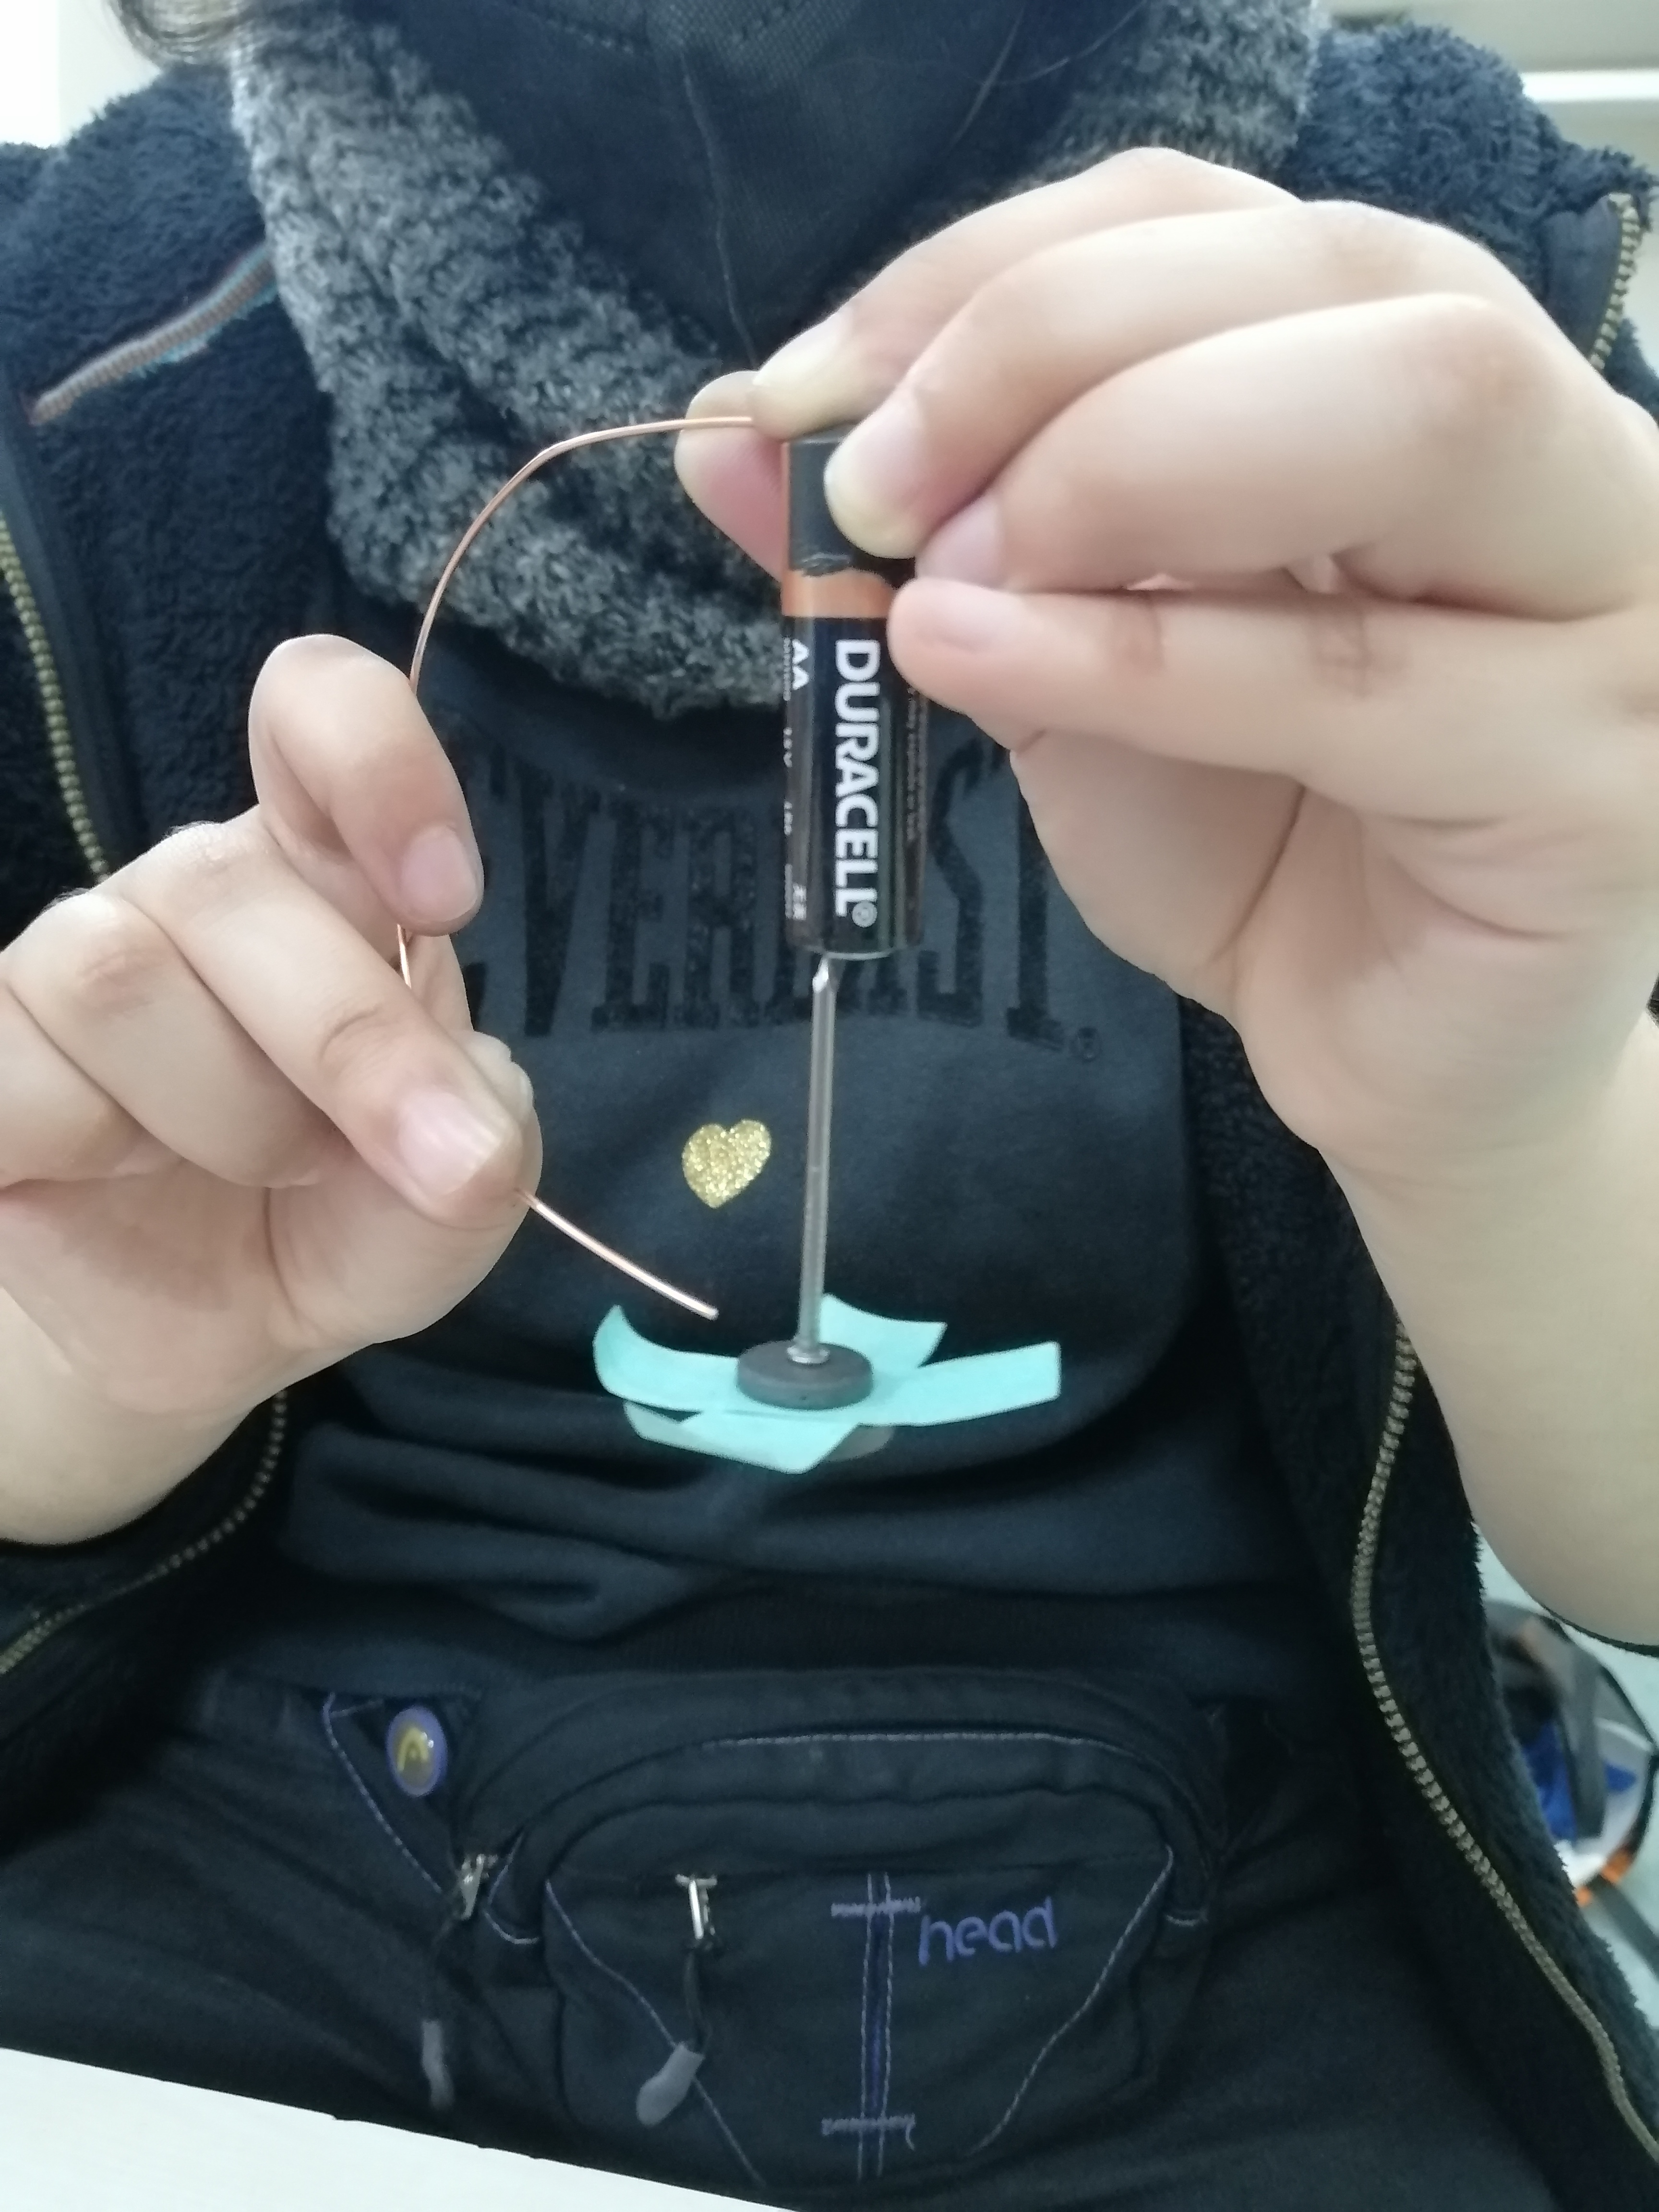
\includegraphics[width=3.5cm, height=4cm]{imag/IMG_20220930_103815.jpg}
\end{Figura}

%%%%%%%%%%%%%%%%%%%%%%%%%%%%%%%%%%%%%%%%%%%%%%%%%%%%%%%%%%




\section*{Experimento 2: Electroimán.}
\textit{Materiales: Pila XL, cable de cobre, tornillo, clavos, cartonero.}

\vspace{-\topsep}
\begin{itemize}
    \setlength{\parskip}{0pt} 
    \setlength{\itemsep}{0pt plus 1pt}
    \item Primero, errollamos el tornillo con el cable de cobre.
    \item Segundo, quitamos el esmalte de los extremos del cable con un cartonero.
    \item Tercero, uno de los extremos del cable lo conectamos al lado positivo, de la pila, y el otro al lado negativo.
    \item Finalmente, probamos nuestro electroimán aproximandolo a un conjunto de clavos.
\end{itemize}
\vspace{-\topsep}

\begin{Figura}
    \centering
    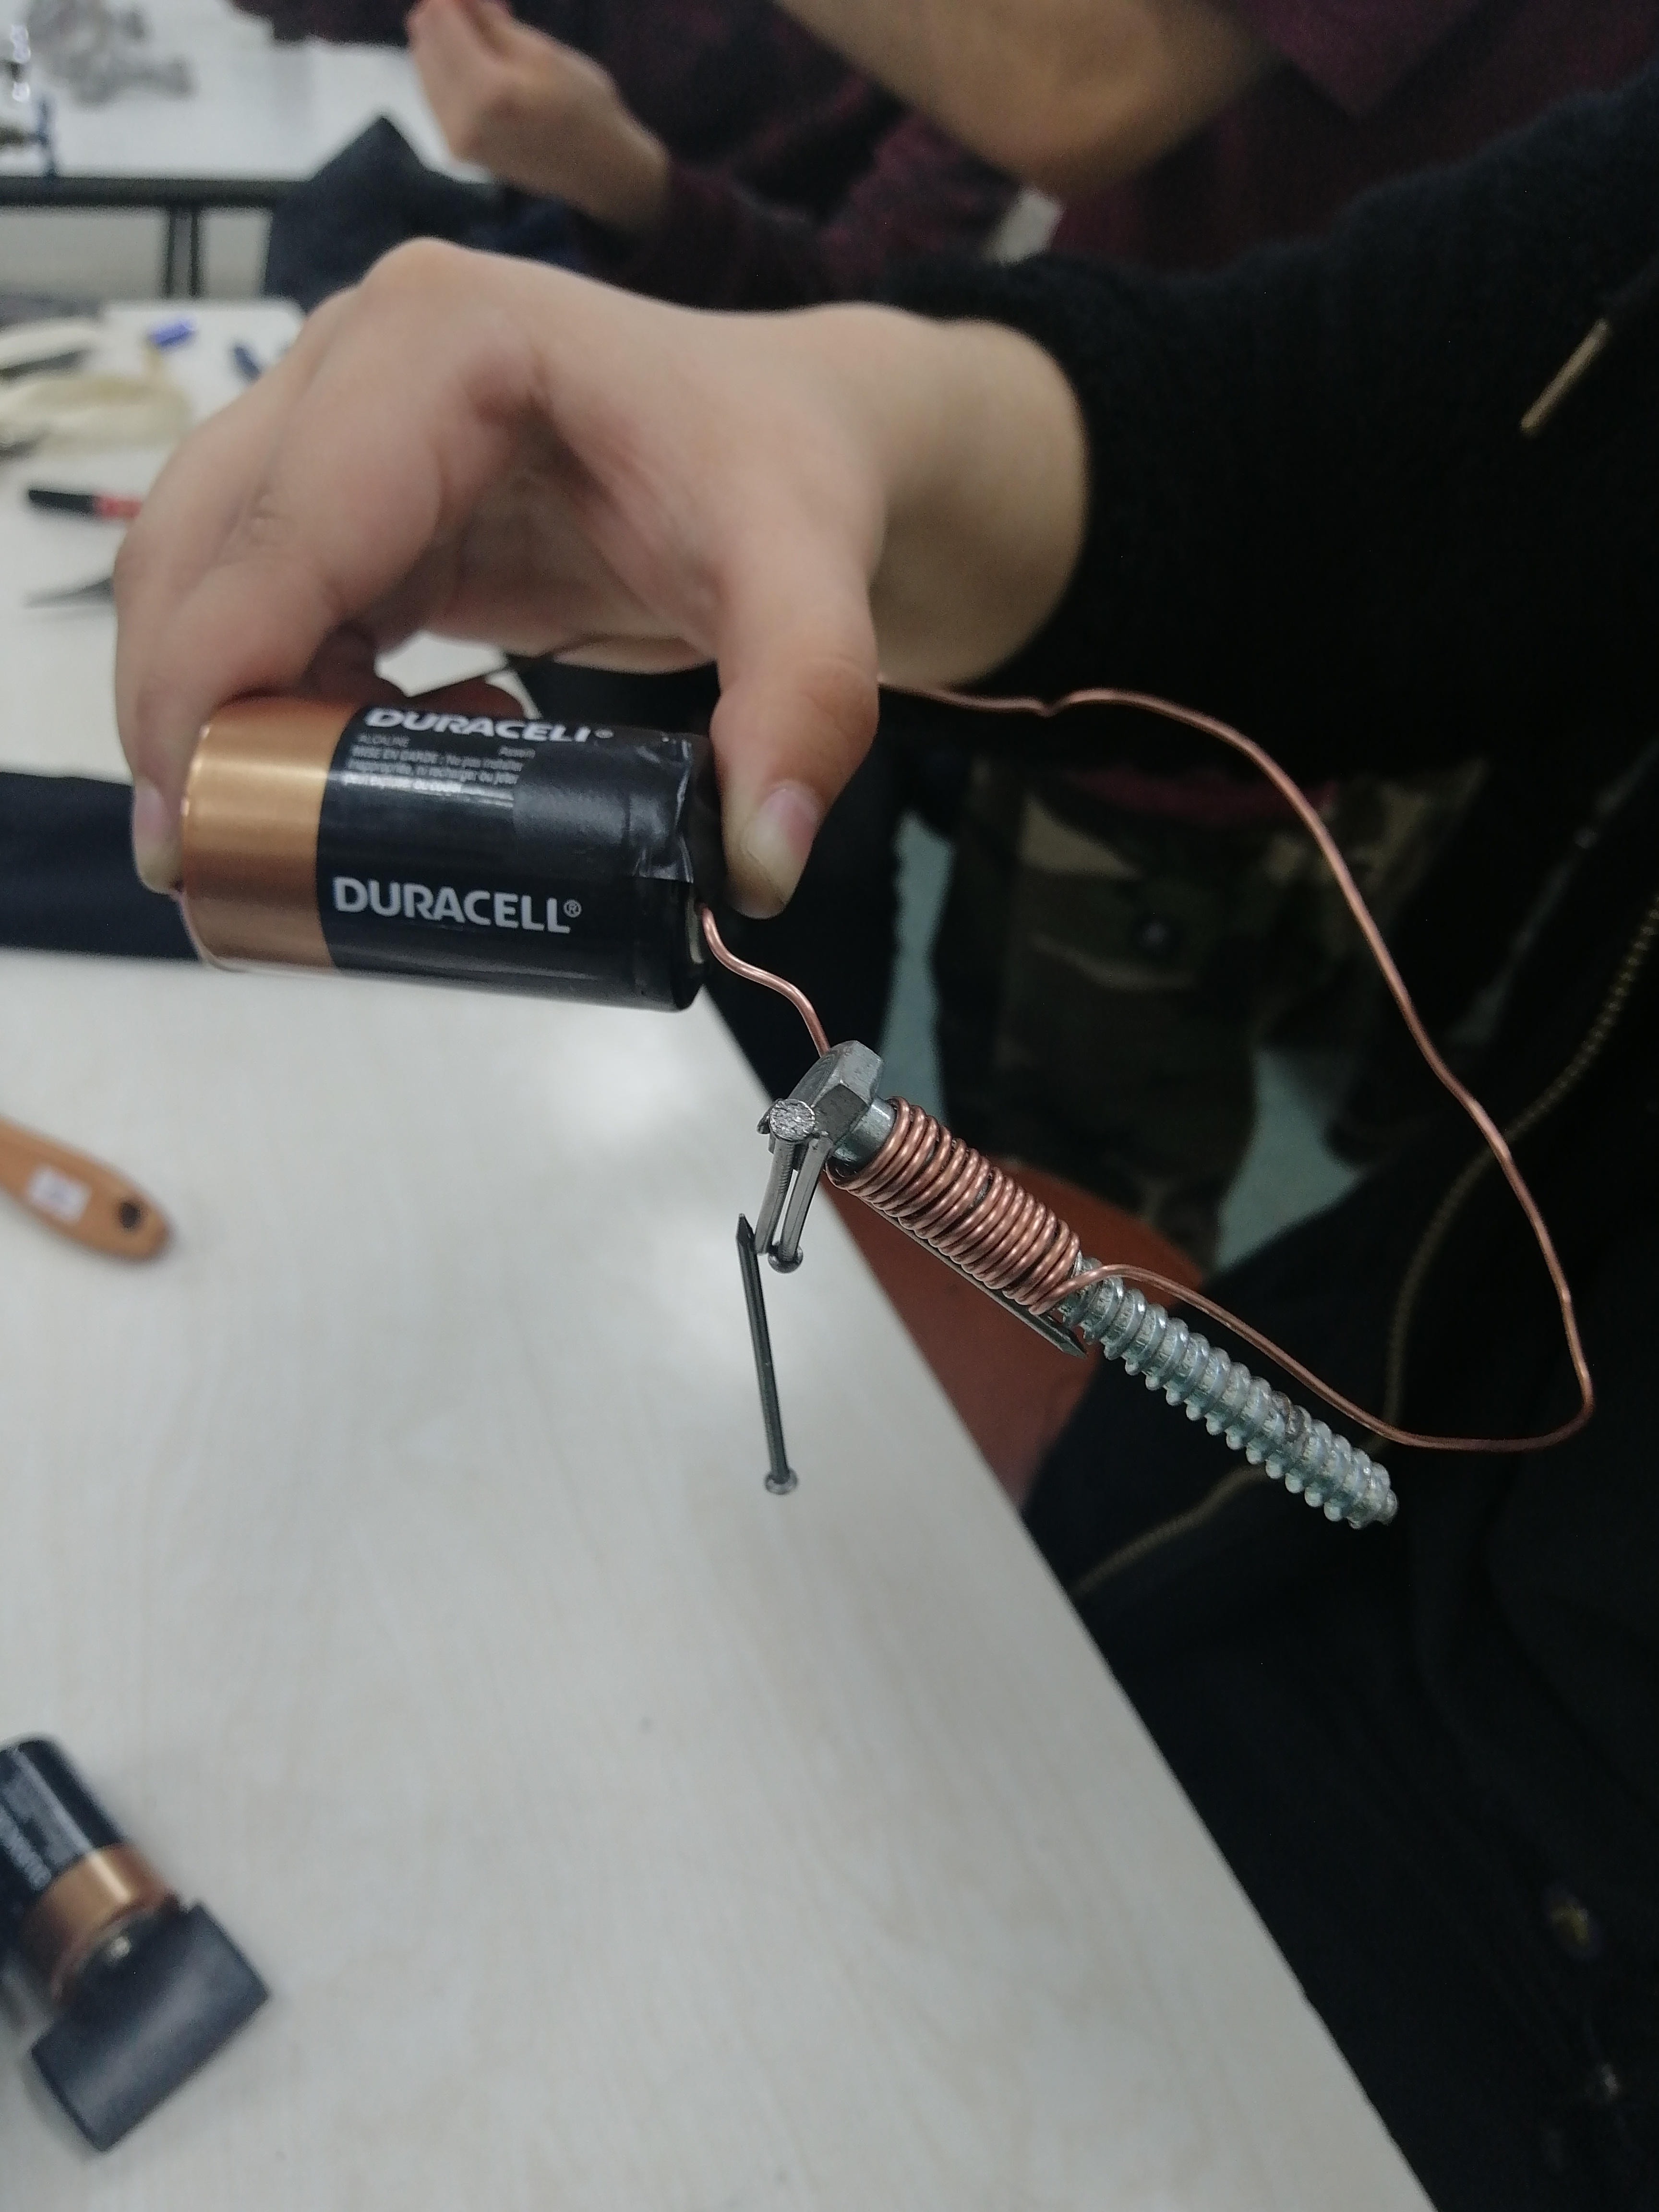
\includegraphics[width=3.5cm, height=4cm]{imag/IMG_20220930_105337.jpg}
\end{Figura}



%%%%%%%%%%%%%%%%%%%%%%%%%%%%%%%%%%%%%%%%%%%%%%%%%%%%%%%%%%%%%%%%%%%%%%%

    
\section*{Experimento 3: Inducción magnética.}
\textit{Materiales: Papel de aluminio, 2 imanes pequeños, recipiente de plástico, hilo de coser.}
\vspace{-\topsep}
    \begin{itemize}
       \setlength{\parskip}{0pt} 
       \setlength{\itemsep}{0pt plus 1pt}
        \item Primero, llenamos el recipiente, hasta la mitad, con agua.
        \item Segundo, con el papel de aluminio, hacemos un mini vaso y lo dejamos sobre el agua.
        \item Tercero, ponemos el hilo entre los dos imanes, formando un péndulo.
        \item Finalmente, hacemos girar nuestro péndulo sobre el mini vaso de aluminio.
    \end{itemize}
\vspace{-\topsep}


\begin{Figura}
    \centering
    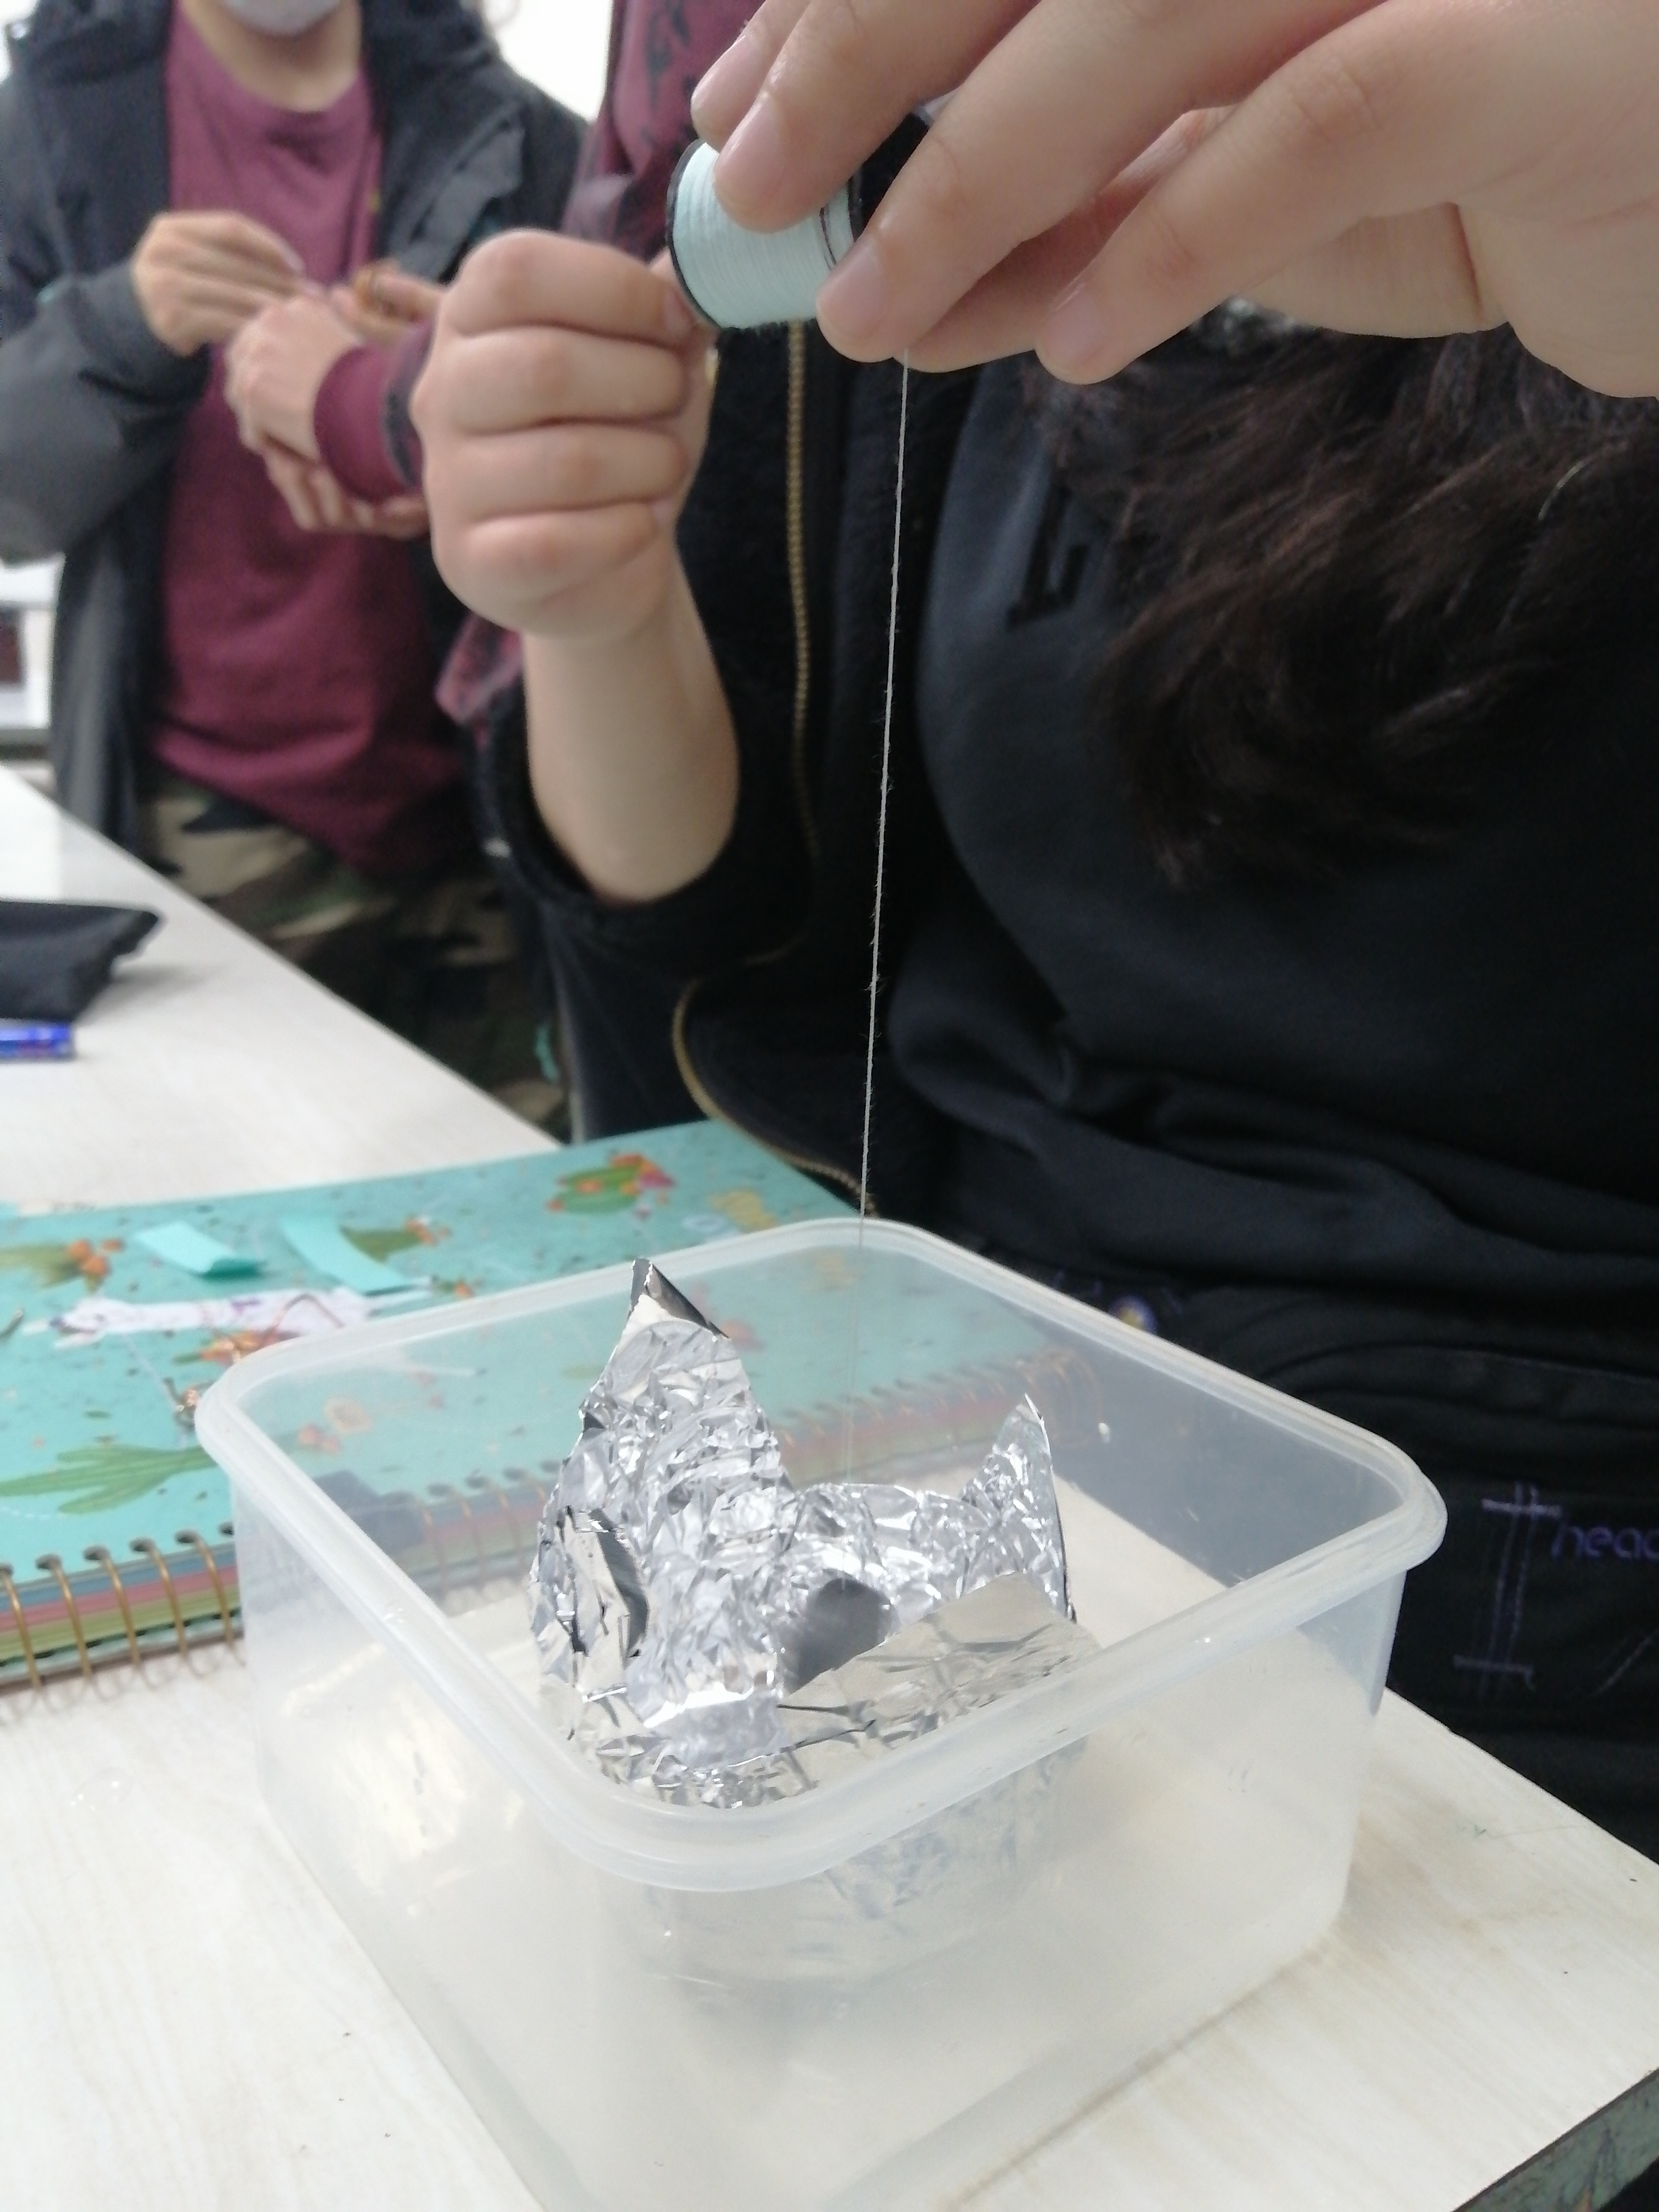
\includegraphics[width=3.5cm, height=4cm]{imag/IMG_20220930_111527.jpg}
\end{Figura}


    
%============Análisis==========================================================
\section*{Análisis}
Analizando a mayor profundidad los resultados de nuestros experimentos, podemos ver que todos están relacionados por la misma rama de la física, la cual es la rama del electromagnetismo, pero definidos por diferentes tópicos.\\
Para el primer experimento, el motor homopolar, podemos ver que cuando conectamos el cable de cobre con el imán, los imanes y el clavo empiezan a dar vueltas, por lo que suponemos que debe haber alguna fuerza que produzca este movimiento, 
este movimiento puede ser explicado con la ley de Lorentz \eqref{eq: Lorentz}.\\
La pila genera un voltaje que hace circular corriente a través del cable de cobre, que después pasa por el imán, luego por el clavo y vuelve a pasar por la pila, por lo que la corriente circula continuamente, además de que 
la velocidad de la carga eléctrica es radial.\\
 Por otro lado lo que genera el campo magnético en nuestro caso son los imanes, los cuales generan un campo magnético vertical en direccion al clavo, ahora tomando en cuenta la dirección de la velocidad 
de la carga eléctrica y la dirección del campo magnético y reemplazandola en \eqref{eq: Lorentz} , tenemos como resultado una fuerza perpendicular que genera un momentum y hace girar el clavo con los imanes. Como nosotros estamos sujetando el cable 
de cobre, lo que giran son los imanes y el clavo. Dependiendo de como coloquemos los imanes, estos pueden girar en sentido horario o antihorario.\\
\vspace{0.3cm}

Para el segundo experimento, el electroimán, vemos que al pasar corriente eléctrica a través de un conductor, es decir, el cable de cobre, se genera un campo magnético muy débil, que luego es aumentado al enrrollar el cable alrededor del tornillo.  Así canalizamos las líneas electromagnéticas hacia un mismo punto, y conseguimos un eletroimán. \\
Notemos que este fenómeno, se relaciona con la ley de Ampére \cite{Ley-de-Ampere}, más especificamente para un solenoide.\\
De su ecuación \eqref{eq: solenoide}, podemos deducir que el campo magnético es proporcional a la cantidad de vueltas que tiene el solenoide, dicho de otra manera, a mayor cantidad de vueltas,  mayor será el campo magnético. \\ 

\vspace{0.3cm}
Para el último experimento vemos que al tener el vaso de aluminio y acercarle los imanes, este no se siente atraído en lo mas mínimo, ya que el aluminio no es un material ferromagnético, pero al hacer suspender los imanes y hacerlos girar, sin que los imanes toquen el vaso, el vaso comienza 
a girar en el sentido que  los imanes. \\ 
Lo que genera este fenómeno es explicado por la ley de Faraday \cite{Ley-de-Faraday}, cuando se hace girar el imán, el  campo magnético varía, generando así una fem\footnote[1]{Fuerza electro motriz}.
Esta fem \eqref{eq: Faraday} cuando se produce al interior de un conductor, en este caso el aluminio,  genera una corriente eléctrica, llamada corrientes de Foucalt \cite{Corrientes-de-Foucault}, las cuales 
causan pequeños circuitos que generan un campo magnético, el cual viene dado por la ley de Lenz \cite{Ley-de-Faraday}.
Entonces tenemos por un lado el campo magnético que generan los imanes, que varía en el espacio cuando los hacemos girar, y por el otro lado el campo magnético que generan las corrientes de Foucalt que se producen en el vaso de aluminio las cuales generan su propio campo magnético. Esos dos campos magnéticos son los que interactúan y hacen mover el vaso de aluminio.



%============Conclusión========================================================
\section*{Conclusión}
En los tres experimentos previamente analizados podemos deducir que: \\ Primero, un imán en presencia de un campo eléctrico puede generar movimiento mecánico. Segundo, al hacer circular corriente por conductores, estos generan un campo magnético. Tercero, vemos que al hacer variar un campo magnético en el tiempo creamos una fuerza electromotriz, la cual a su vez, cuando está dentro de un conductor, genera corrientes que al mismo tiempo producen un nuevo campo magnético,
el cual se opone a el campo magnético inicial. \\ Gracias a la Ley de Lorentz, la Ley de Ampére, la Ley de Faraday, Ley de Lenz y a las corrientes de Foucalt, nosotros somos capaces de explicar y entender estos experimentos, sin aquellos grandes descubrimientos nuestra vida cotidiana no sería la misma, ya que no podriamos utilizar cocinas de inducción, motores, autos y todo lo que conlleva con esto.





\begin{thebibliography}{5}
    \bibitem{Ley-de-Lorentz}  Ley de Lorentz. (s. f.). Fisicalab. Recuperado 7 de octubre de 2022, 
    de \url{https://www.fisicalab.com/apartado/ley-de-lorentz}
    \bibitem{Ley-de-Ampere}Ley de Ampère. (s. f.). Fisicalab. Recuperado 8 de octubre de 2022, 
    de \url{https://www.fisicalab.com/apartado/ley-de-ampere}
    \bibitem{Ley-de-Faraday} \textbf{D. Halliday; R. Resnick; K. S. Kane.} \textit{Física Vol. 2.} (Cap.36), Compañía Editorial Continental, S.A. de C.V. 3º Edición, 1994
    \bibitem{Corrientes-de-Foucault} Eddy Current, que es y como detectarla. - Frigochiller. (2020, 31 marzo). Frigochiller - Mantenimiento y reparacion de Chillers. Recuperado 8 de octubre de 2022, 
    de \url{https://frigochiller.com/corriente-de-foucault/}
\end{thebibliography}
\end{multicols*}























\end{document}